\section{Interaktion med sociale robotter}
\label{InteraktionSocialeRobotter}
%
Inden der dykkes ned i hvilke parametre, der har indflydelse på hvordan interaktionen med sociale robotter perciperes og accepteres, vil nogle mere generelle tendenser blive diskuteret. Det dækker blandt andet over køns-, alders- samt kulturelleforskelle i henhold til synet på sociale robotter. Dernæst gives der nogle eksempler på, hvordan relaterede studier har målt brugerens perception og accept af sociale robotter.
%
\subsection{Generelle tendenser}
\label{InteraktionSocialeRobotterGenerelleTendenser}
%
I den vestlige verden er vi i langt mindre grad villige til at acceptere sociale robotter end hvad der eksempelvis er tilfældet i Japan, \parencite[s. 28]{PDF:InTheCompanyofRobots}. Det skyldes, ifølge \textcite[s. 28]{PDF:InTheCompanyofRobots}, at der er en indgroede frygt for maskiner og følelsen af manglende kontrol, hvilket ikke er tilfældet i den Japanske kultur, som åndeliggøre robotter. At mennesker i den vestlige verden frygter robotter kan, blandt andet, retfærdiggøres med at i 2012 angav 87 \% af borgerne i Europa, at de aldrig har været i kontakt med en robot, hverken i hjemmet eller på ens arbejdsplads, \parencite[s. 40]{PDF:PerceptionAcceptance}. I en undersøgelse, beskrevet af \textcite[s. 41]{PDF:PerceptionAcceptance}, fremgår det at synet på robotter ikke har ændret sig de sidste 35 år. Når robotterne, ved brug af tegninger, visualiseres så minder de i høj grad om robottypen: \textit{Non assistive robots}, illustreret på \autoref{fig:CategorizationOfRobots}. Endvidere tyder det på, at Europærer frygter, at de vil miste deres job til robotten og at robotten er til for at erstatte mennesket, \parencite[s. 22]{PDF:RobotShiftFromIPtoSR}.   

Derudover er der en tendens til, at mænd i højere grad perciperer robotten som menneskeagtig sammenlignet med kvinder, som i langt højere grad perciperer robotten som en maskine, \parencite[s. 28]{PDF:InTheCompanyofRobots}. Ifølge \textcite[s. 1479]{PDF:ExploringInfluencingVariable}, perciperer mænd robotter som værende mere brugbare, de har større intention om at bruge dem og de er mere villige til at acceptere robotter end kvinder er.  

Ydermere argumenterer \textcite[s. 2]{PDF:SharingALifeHarvey} for, at den ældre population i højere grad accepterer sociale robotter, sammenlignet med den yngre population. Det antages, at en af årsagerne til det formentlig skyldes, at der anvendes sociale robotter i ældreplejen eksempelvis til mindske følelsen af ensomhed, \fullref{EksisterendeSocialeRobotter}. I mere praktiske situation, som eksempelvis rengøring, tøjvask og lignende, foretrækker ældre robotter fremfor mennesker, hvorimod hvis opgaverne er omsorgsrelateret foretrækkes mennesker, \parencite[s. 22]{PDF:RobotShiftFromIPtoSR}.

\subsection{Parametre, der har indflydelse på accept og interaktion med sociale robotter}
\label{InteraktionSocialeRobotterParametre}
%
\textcite[s. 1477]{PDF:SharingALifeHarvey} opstiller tre forskellige problemstillinger, der bør overvejes når brugerens accept af en social robot undersøges. I de følgende afsnit undersøges hvilke parametre, der har indflydelse på brugerens accept i forhold til de tre problemstillinger: 
%
\begin{quotation}
\textit{
  \begin{enumerate}
  \item the likely positive or negative consequences of the behavior
  \item the approval or disapproval of the behavior by respected individuals or groups, and
  \item the factors that may facilitate or impede performance of the behavior,
\end{enumerate}}
\textcite[s. 1477]{PDF:SharingALifeHarvey}.\blankline
\end{quotation}
\noindent
%
Overvejelserne afspejler henholdvist brugerens evaluering af robotten, hvilke sociale normative overbevisninger, der tilskrives robotten ved brug samt hvilke kontekstuelle faktorer, der spiller ind ved brug, \parencite[s. 1477]{PDF:SharingALifeHarvey}. Baseret på \textcite[ss. 1477-1478]{PDF:SharingALifeHarvey} tyder det på, at der er to overordnede kategorier af parametre, som har indflydelse på den første problemstilling: Utilitaristiske og hedoniske parametre. Førstnævnte dækker over det praktiske og anvendelige aspekt ved at interagere med en social robot, hvor sidstnævnte relateres til brugerens oplevelse af at anvende den sociale robot, \parencite[s. 1476]{PDF:SharingALifeHarvey}.

I følgende to afsnit vil de utilitaristiske og hedoniske parametre undersøges nærmere, hvorefter de sociale normative overbevisninger og efterfølgende hvilke parametre, der har indflydelse på præstationsevnen, undersøges.
%   
\vfill
\subsubsection*{Utilitaristiske parametre}
\label{InteraktionSocialeRobotterParametreUtilitarian}
%
Som nævnt dækker utilitaristiske parametre over det praktiske og anvendelige aspekt ved at interagere med en social robot. Derudover har disse parametre ligeledes indflydelse på den specifikke adfærd. I følgende afsnit belyses hvilke parametre, der har indflydelse på det praktiske såvel som det anvendelige aspekt. Der tages primært udgangspunkt i \textcite[s. 1477]{PDF:SharingALifeHarvey}.
%
\begin{figure}[H]
\centering
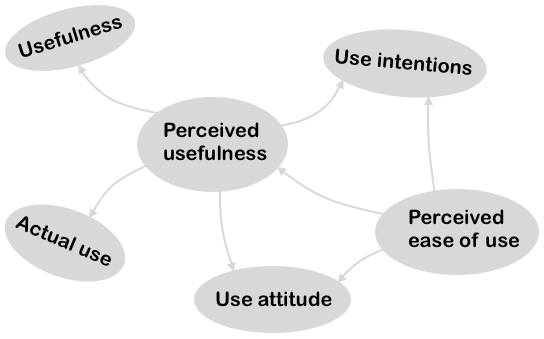
\includegraphics[width = 0.75\textwidth]{Figure/UtilitarianParameters} 
\caption{Sammenhængen mellem de seks forskellige parametre, der har indflydelse på det praktiske og anvendelige aspekt. Pilene indikerer hvilken retning indflydelsen er mellem to parametre.}
\label{fig:UtilitarianParameters}
\end{figure}
\noindent 
%
Baseret på \textcite[s. 1477]{PDF:SharingALifeHarvey} defineres \textit{usefulness} som værende brugerens overbevisning om, at robotten vil forbedre de daglige aktiviteter. Ifølge \textcite[s. 11]{PDF:SharingALifeHarvey} tyder det på, at \textit{usefulness} er en vigtig parametre, der kan bidrage til langtidssigtet forhold mellem bruger og robot. \textit{Ease of use} defineres som værende brugerens overbevisning om, at det nemt at anvende robotten. Derudover argumenterer \textcite[s. 1477]{PDF:SharingALifeHarvey} for, at i situationer hvor robotten skal indgå i en social interaktion med mennesker, er det nødvendigt at robotten gengiver menneskeagtige træk, for at brugeren føler sig komfortabel nok til at indgå i interaktionen. Robottens evne til at tilpasse sig den sociale kontekst afhængigt af brugeres behov, defineres som \textit{perceived adaptability}. Ifølge \textcite[s. 1477]{PDF:SharingALifeHarvey}, har \textit{perceived adaptability} indflydelse på \textit{perceived usefulness}, \textit{use attitude}, \textit{use intentions}, som er repræsenteret på \autoref{fig:UtilitarianParameters}. Derudover har \textit{perceived adaptability} indflydelse på \textit{enjoyment}. Ydermere tyder det på at \textit{intelligence}, har en effekt på hvor realistiske robotten perciperes, \parencite[s. 1477]{PDF:ExploringInfluencingVariable}.   
%
\subsubsection*{Hedoniske parametre}
\label{InteraktionSocialeRobotterParametreHedonic}
%
Som nævnt dækker hedoniske parametre over brugerens oplevelse af at anvende den sociale robot. Derudover har disse parametre ligeledes indflydelse på den specifikke adfærd. I følgende afsnit belyses hvilke parametre, der har indflydelse på det dette. Der tages primært udgangspunkt i \textcite[ss. 1477-1478]{PDF:SharingALifeHarvey}. På \autoref{fig:HedonicParameters} illustreres forskellige parametre, samt deres indbyrdes forhold.
%
\begin{figure}[H]
\centering
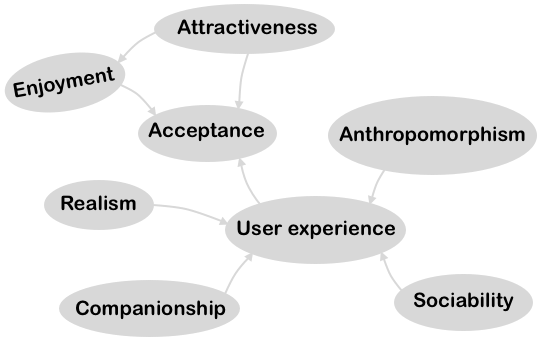
\includegraphics[width = 0.75\textwidth]{Figure/HedonicParameters} 
\caption{Sammenhængen mellem de otte forskellige parametre, der har indflydelse på brugerens oplevelse. Pilene indikerer hvilken retning indflydelsen er mellem to parametre.}
\label{fig:HedonicParameters}
\end{figure}
\noindent 
%
Baseret på \textcite[s. 1477]{PDF:ExploringInfluencingVariable} har både \textit{enjoyment}, der defineres som værende følelsen af fornøjelse eller glæde forbundet med brug, og \textit{attractiveness}, der defineres som værende den positive evaluering af robottens udseende, på flere af de parametre gengivet på \autoref{fig:UtilitarianParameters}. \textit{Enjoyment} har indflydelse på \textit{ease of use}, \textit{use attitude} samt \textit{use intentions}. Derimod har \textit{attractiveness} indflydelse på \textit{usefulness} og \textit{ease of use}. \blankline 
%
Antropomorfisering defineres som værende evnen til at tilskrive naturfænomener, guder, overnaturlige væsner og dyr menneskelige egenskaber, såsom følelser og motiver, \parencite{WEB:DefAntropomorisering}. Dog defineres antropomorfisering i HRI sammenhæng, som værende evnen til at tildele og beskrive objekter med menneskelige egenskaber, for at rationalisere objektets adfærd, \parencite[s. 1478]{PDF:ExploringInfluencingVariable}. Ifølge \textcite[s. 1478]{PDF:ExploringInfluencingVariable} har anthropomorfisme indflydelse på \textit{usefulness}, \textit{use attitude} samt \textit{use intention}, som er repræsenteret på \autoref{fig:UtilitarianParameters}. Derudover har \textit{anthropomorphism} ligeledes indflydelse på \textit{attitude toward robots}, \textit{social influence} samt \textit{companionship}. Ifølge \textcite[s. 19]{PDF:CloseButNotStuck} resulterer antropomorfisering i, at mennesket betragter en social robot som en social enhed, hvorfor robotten behandles som et menneske.

Der er forskellige årsager til at mennesker antropomorfiserer sociale robotter. Antropomorfisering kan forekomme i situationer hvor mennesket oplever en manglende kontrol og usikkerhed, hvor mennesket i højere grad har en tendens til at antropomorfisere sociale robotter, for at kunne forstå, kontrollere samt forudse robottens adfærd, \parencite[s. 1478]{PDF:ExploringInfluencingVariable}. Dette høre under \textit{effectance motivation}, der defineres som værende ønsket om effektivt at kunne interagere med ens omgivelser, \parencite[s. 62]{PDF:EffectsOfAnticipatedHRI}.

Derudover har mennesker med en teknologisk baggrund en tendens til at tildele robotten sin egen personlighed, hvilket ikke er tilfældet med mennesker uden teknologisk baggrund, \parencite[s. 19]{PDF:CloseButNotStuck}. I tillæg argumenterer \textcite[s. 2]{PDF:SharingALifeHarvey} for, at desto mere antropomorfisering brugeren oplever, desto bedre er evalueringen af robotten, desto mere fornøjet er de med interaktionen og desto større er chancen for at de oplever robotten som en ledsager.

Ifølge \textcite[s. 61]{PDF:EffectsOfAnticipatedHRI} har ensomme mennesker en stærk tendens til at antropomorfisere kæledyr og teknologiske objekter, såsom robotter. Det skyldes, at mennesket har et behov for både tilknytning og et tilhørsforhold. Dette hører under \textit{sociality motivation}, der defineres som værende ønsket og behovet for at skabe en social relation til andre, \parencite[s. 61]{PDF:EffectsOfAnticipatedHRI}. I det henseende vil en robot med et mere livagtigt udtryk perciperes som værende en venlig ledsager, \parencite[s. 1478]{PDF:ExploringInfluencingVariable}. Dette gengives som \textit{companionship}, der defineres som brugerens perciperede mulighed for at bygge et forhold til robotten. \textit{Companionship} er illustreret på \autoref{fig:HedonicParameters} og udover at have indflydelse på \textit{user experience}, har \textit{companionship} indflydelse på den vedvarende interaktion med robotten. \blankline
%
Baseret på \textcite[s. 1478]{PDF:ExploringInfluencingVariable} tyder det på, at \textit{realism} kan forbedre HRI og har dermed indflydelse på \textit{user experience}, \autoref{fig:HedonicParameters}. En robots \textit{realism} afspejler i hvilken grad brugeren tro på, at robotten reagerer og opfører sig realistisk. Desto mere realistisk robotten perciperes, desto mere intelligent perciperes den, \parencite[s. 1478]{PDF:ExploringInfluencingVariable}. 

\textit{Sociability} defineres som værende brugerens overbevisning om hvorvidt robotten besidder de sociale, emotionelle samt kognitive færdigheder, der er nødvendige for en succesfuld tilvænning af robotten, \parencite[s. 1478]{PDF:ExploringInfluencingVariable}. Denne parameter har, ifølge \textcite[s. 1478]{PDF:ExploringInfluencingVariable}, ligeledes indflydelse på \textit{use attitude} og \textit{usefulness}.\blankline
%
I henhold til teknologier i lufthavne argumenterer \textcite[s. 352]{PDF:TheImpactOfTraveler} for, hvorfor der bør tages højde for \textit{hedonic} parametre. En stor del af den teknologi, som kan findes i lufthavne bygger primært på \textit{utilitarian} parametre, hvilket formentlig har været årsagen til en dårlig brugeroplevelse. For at forbedre dårlige oplevelser, blandt andet ved lange ventetider ved sikkerhedskontrollen, har lufthavne forsøgt at foretage nogle tiltag, der skal gøre oplevelsen bedre, hvilket eksempelvis kommer til udtryk ved et øget brug af smartphone applikationer. Derudover understreger \textcite[s. 352]{PDF:TheImpactOfTraveler}, at det er nødvendigt at skabe fornøjelige lufthavns oplevelser. Fornøjelighed gengives på \autoref{fig:HedonicParameters}, som \textit{enjoyment}.
%

\subsubsection*{Sociale normer}
\label{InteraktionSocialeRobotterParametreSocialeNormer}
% 
I henhold til problemstilling 2: \textit{the approval or disapproval of the behavior by respected individuals or groups}, fremsat af \textcite[s. 1477]{PDF:SharingALifeHarvey}, vil følgende afsnit undersøge hvilke parametre, der har indflydelse på det.\blankline
%
De sociale normer dækker over de synspunkter mennesket har i relation til deres egen adfærd og dækker ydermere de synspunkter og regler, der er gældende for en gruppe for hvorvidt en bestemt adfærd er passende eller upassende, \parencite[s. 1478]{PDF:ExploringInfluencingVariable}. Ifølge \textcite[s. 1478]{PDF:ExploringInfluencingVariable} dækker de sociale normer over \textit{social influence} og \textit{image}. \textit{Social influence} er karakteriseret ved brugerens perception af hvad andre tænker omkring brugen af robotten. Denne parameter har indflydelse på \textit{usefulness}, \textit{ease of use}, \textit{use attitude}, \textit{use intention} samt \textit{actual use}, \parencite[s. 1478]{PDF:ExploringInfluencingVariable}, jævnfør \autoref{fig:UtilitarianParameters}. Det er særligt mennesker i ens tætte omgangskreds; familie, partner og venner, hvis mening har indflydelse på hvorvidt en bestemt teknologi vil blive brugt, i dette tilfælde en social robot, \parencite[s. 1478]{PDF:ExploringInfluencingVariable}. 

\textit{Image} karakteriseres ved brugerens overbevisning om at interaktionen med robotten kan lede til større anerkendelse og social status blandt ens omgangskreds, \parencite[s. 1478]{PDF:ExploringInfluencingVariable}. Derudover har \textit{image} indflydelse på \textit{perceived usefulness}, illustreret på \autoref{fig:UtilitarianParameters}.\blankline
%
I relation til sociale normer og tilnærmelsesvis \textit{social influence} undersøger \textcite{PDF:HowSocialDistanceShapesHRI}, hvilken indflydelse \textit{social distance} har på HRI. \textit{Social distance} referer til hvilken grad mennesker perciperer manglende intimitet grundet forskellige egenskaber såsom etnicitet, race, religion, beskæftligelse, \parencite[s. 784]{PDF:HowSocialDistanceShapesHRI}. \textit{Social distance} dækker over to forskellige parametre; \textit{social structural distance} og \textit{physical distance}.

\textit{Social structural distance} referer til mennesket perception af og adfærd rettet mod andre, som er afhænger af hvordan mennesket kategoriserer andre, særligt i forhold til deres kompetance og varme, \parencite[s. 784]{PDF:HowSocialDistanceShapesHRI}. Derudover kategoriseres mennesker afhængigt af deres indbyrdes forhold, er der forskel i status, foregår interaktionen som samarbejde eller som en konkurrence. \textit{Social structural distance} kan inddeles i yderligere to kategorier; \textit{power distance} og \textit{task distance}. Førstnævnte har stor indflydelse på den individuelle's adfærd og perception afhængigt af forholdet til interaktionspartneren, som afhænger af personligheder, roller og deres individuelle sociale klasse, \parencite[s. 784]{PDF:HowSocialDistanceShapesHRI}. \textit{Task distance} referer til at mennesker afhænger af hinanden for at opnå deres mål, det kan enten komme positivt til udtryk når mennesker samarbejder for opnår deres fælles mål, eller negativt når mennesker konkurrerer mod hinanden og når de forhindre hinanden i at opnå deres individuelle mål, \parencite[s. 784]{PDF:HowSocialDistanceShapesHRI}. 

\textit{Physical distance} kan også beskrives som \textit{proxemic distance} og referer til den fysiske adskillelse mellem mennesker, \parencite[s. 784]{PDF:HowSocialDistanceShapesHRI}. Der opstår både bedre kommunikation mellem mennesker og den individuelle vil være i stand til at løse egne opgave bedre, \parencite[s. 785]{PDF:HowSocialDistanceShapesHRI}.\blankline
%
\textcite[s. 794]{PDF:HowSocialDistanceShapesHRI} undersøger forholdet mellem \textit{power distance} og \textit{proxemic distance} i forhold til HRI. \textit{Power distance} udtrykkes ved at robotten enten agerer som \textit{supervisor} eller som \textit{subordinate}, hvor \textit{proxemic distance} udtrykkes ved at afstanden mellem robot og menneske er lille eller stor. Baseret på disse resultater tyder det på, at \textit{user experience} blev bedre når interaktionen foregik med en \textit{supervisor} robot tæt på og når interaktionen foregik med en \textit{subordinate} robot langt væk, \parencite[s. 785]{PDF:HowSocialDistanceShapesHRI}. Dog finder \textcite[s. 785]{PDF:HowSocialDistanceShapesHRI}, at præstationen i opgaven blev forværret desto tætter robotten var på testpersonen, uafhængigt af \textit{power distance}. 

Derudover finder \textcite[s. 785]{PDF:HowSocialDistanceShapesHRI}, at \textit{user experience} blev forbedret når robotten konkurrerede med testpersonen tæt på og når robotten samarbejde med testpersonen langt væk, hvilket var imod forventningen, \parencite[s. 785]{PDF:HowSocialDistanceShapesHRI}.   
%
\subsubsection*{Indflydelse på præstationsevnen}
\label{InteraktionSocialeRobotterParametrePraestation}
%
I henhold til problemstilling 3: \textit{the factors that may facilitate or impede performance of the behavior}, fremsat af \textcite[s. 1477]{PDF:SharingALifeHarvey}, vil følgende afsnit undersøge hvilke parametre, der har indflydelse på præstationsevnen.\blankline
%
\textit{Control beliefs} referer til brugerens overbevisning om hvilke ressourcer, muligheder og forhindringer, der er tilstede eller fraværende og som vil have en positiv eller negativ indflydelse på præstationsevnen, \parencite[s. 1478]{PDF:ExploringInfluencingVariable}. \textit{Control beliefs} kan inddeles i tre kategorier, som alle har indflydelse på \textit{user acceptance}: \textit{Perceived behavioral control}, \textit{anxiety} og \textit{experience}, begge rettet mod robotter, \parencite[s. 1478]{PDF:ExploringInfluencingVariable}. 

\textit{Perceived behavioral control} defineres som værende brugerens perciperede oplevelse af hvor let eller svært det var at interagere med robotten, \parencite[s. 1478]{PDF:ExploringInfluencingVariable}. \textit{Perceived behavioral control} har indflydelse på \textit{perceived ease of use}, \textit{use intentions} samt \textit{actual use}. \textit{Anxiety} rette mod robotter defineres som værende ængstelige eller andre negative emotioner forbundet med HRI og som forværres afhængigt at tidligere oplevelser, \parencite[s. 1478]{PDF:ExploringInfluencingVariable}. \textit{Anxiety} har en negativ effekt på \textit{perceived ease of use}, men \textit{anxiety} kan reduceres med \textit{enjoyment}, \parencite[s. 1478]{PDF:ExploringInfluencingVariable}. 

\textit{Experience} med robotter defineres som den opnåede oplevelse med robotter både direkte, i form af HRI, og indirekte via et medie, såsom nyhedsartikler og science-fiction film, \parencite[s. 1479]{PDF:ExploringInfluencingVariable}. Som nævnt i \fullref{InteraktionSocialeRobotterGenerelleTendenser}, har 87 \% af borgerne i Europa aldrig indgået i en interaktion med en robot, hvorfor det antages at den direkte oplevelse med robotter er begrænset, hvert fald i Europæiske lande.

Tidligere erfaring med robotter har, ifølge \textcite[s. 1479]{PDF:ExploringInfluencingVariable}, en positiv effekt på: \textit{Usefulness}, \textit{ease of use}, \textit{attitude towards robots}, \textit{use intention} samt \textit{actual use}. I henhold til tidligere erfaringer med robotter, undersøger \textcite{PDF:CloseButNotStuck} hvorvidt \textit{online community} og erfaring med \textit{avatars}, har en indflydelse på evnen til at antropomorfisere og acceptere robotter. \textit{Community} defineres som forholdet mellem individet og den sociale struktur de tilhører, \parencite[ss. 20-21]{PDF:CloseButNotStuck}. Det essentielle ved \textit{community} dækker over support, \textit{sociability}, information, dannelse af social identitet og tilhørsforhold, \parencite[s. 21]{PDF:CloseButNotStuck}. Det eneste der, adskiller \textit{community} fra et \textit{online community} er, at sidstnævnte foregår på virtuelt. \textcite[s. 25]{PDF:CloseButNotStuck} fandt de testpersoner, som enten var en del af \textit{online community} eller mere involveret med \textit{avatars}, i højere grad var i stand til at genkende menneskelige træk ved robotten, sammenlignet med testpersoner uden disse erfaringer. Ydermere fandt \textcite[s. 26]{PDF:CloseButNotStuck} at testpersoner, som enten var en del af \textit{online community} eller mere involveret med \textit{avatars}, begge var mere villige til at acceptere robotter, som en del af deres sociale og fysiske miljø.  
%

\subsection{Bevægelsesmønstre og udseende}
\label{InteraktionSocialeRobotterParametreBevaegelsesmoenstre}
%
Som nævnt i \fullref{InteraktionSocialeRobotterGenerelleTendenser} forekommer der store kulturelle forskelle i forhold til hvordan sociale robotter perciperes. Ikke nok med det, forekommer der ligeledes store kulturelle forskelle i hvordan robotter bør bevæge sig, blandt andet i forhold til hvor tæt de må komme på. Først vil afstanden mellem robot og menneske blive diskuteret, og derefter hvilken hastighed robotten bør bevæge sig med. 

\subsubsection*{Afstand mellem robot og menneske}
\label{InteraktionSocialeRobotterParametreBevaegelsesmoenstreAfstand}
%
Ifølge \textcite[s. 178]{PDF:HowMayIServeYou} er den intime grænse for hvor tæt et andet menneske, tætte venner og familie, må komme på en mellem 20 cm og 30 cm for syd europærer og japanere. Hvorimod denne grænse for amerikanere og nord europæer er 46 cm til 122 cm. Ydermere har mennesker, der er opvokset i et landdistrikt ligeledes behov for en øget intim grænse, modsat mennesker, der er opvokset i bymiljøer, \textcite[s. 178]{PDF:HowMayIServeYou}. Endvidere tyder det på, at kvinder normalvis er tættere på hinanden og vendt mere direkte ansigt-til-ansigt, sammenlignet med mænd, \parencite[s. 178]{PDF:HowMayIServeYou}. Det må derfor antages at kvinder, har en mindre intim grænse end mænd.

I undersøgelsen foretaget af \textcite{PDF:HowMayIServeYou}, undersøger de blandt andet hvor tæt en robot må komme før den overskrider den intime grænse, afhængigt af indgangsvinkel: Frontal, højre eller venstre. Robotten holdte en afstand svarende til 50 cm $\pm$ 10 cm. I den første undersøgelse foretaget af \textcite[s. 174]{PDF:HowMayIServeYou}, angav 76 \% testpersonerne at afstanden mellem dem og robotten var \textit{about right}, 19 \% angav at afstanden var for stor og 5 \% angav at robotten kom for tæt på. I den anden undersøgelse foretaget af \textcite[s. 175]{PDF:HowMayIServeYou}, angav 53 \% af testpersonerne, at når robotten nærmede sig frontalt, at den kom for tæt på, 27 \% angav at afstanden var \textit{about right} og 20 \% angav af afstanden var for stor. Da robotten nærmede sig fra venstre, angav 80 \% af testpersonerne at det var \textit{about right} og 20 \% angav at afstanden var for stor. Da robotten nærmede sig fra højre, angav 60 \% af testpersonerne at afstanden var \textit{about right} og 40 \% angav at afstanden var for stor. I alle tilfælde foregår interaktionen mellem robotten og et siddende menneske.

I henhold til hvilken retning robotten skal nærme sig testpersonerne med fremgår det, at 59 \% foretrækker at robotten nærmer sig fra højre, 28 \% foretrækker venstre og 13 \% foretrækker frontalt, \parencite[s. 175]{PDF:HowMayIServeYou}. Lignende tendens går igen ved hvor praktisk og komfortabelt testpersonerne vurder interaktionen, \parencite[ss. 175-176]{PDF:HowMayIServeYou}. Der skal dog tages højde for kønsforskelle, da en del af kvinderne faktisk foretrækker at robotten nærmer sig frontalt, hvilket formentlig hænger sammen med at kvinder i højere grad interagerer med hinanden ansigt-til-ansigt, sammenlignet med mænd, \parencite[s. 178]{PDF:HowMayIServeYou}. Dog argumenterer \textcite[s. 178]{PDF:HowMayIServeYou} for, at den frontale indgangsvinkel opleves som værende ukomfortabel, upraktisk, truende og konfronterende, hvorfor det bør undgåes. I det henseende kommenterer \textcite[s. 178]{PDF:HowMayIServeYou} at i situationer, hvor der er en 45$^{\circ}$s vinkel mellem to samtale partnere, vil følelser som aggression og konfrontation være reduceret. Derudover skal der tages højde for at 94 \% af testpersonerne er højrehåndede, hvilket formentlig er årsagen til at størstedelen af testpersonerne foretrækker at robotten nærmer sig fra højre, \parencite[s. 175]{PDF:HowMayIServeYou}.\blankline
%
En anden undersøgelse, der blandt andet fokuserer på afstanden mellem robot og menneske, er foretaget af \textcite{PDF:HumanRobotEmodiedInteraction}. Der differentieres mellem fire forskellige afstande, som er gældende for menneske-menneske interaktion. \textit{Intimate distance} denne afstand går direkte fra kroppen til omkring 45 cm fra kroppen, og generelt beregnet til direkte fysisk kontakt eller privat interaktion \parencite[s. 165]{PDF:HumanRobotEmodiedInteraction}. Dernæst er \textit{personal distance}, som går fra 45 cm til 1.2 m, denne afstand gør sig gældende for interaktion med familie og venner eller ved organiserede interaktion, som opstår når mennesker står i kø, \parencite[s. 165]{PDF:HumanRobotEmodiedInteraction}. Den tredje afstand er \textit{social distance}, som går fra 1.2 m til 3.5 m og som er beregnet til mere formelle og arbejdsrelateret interaktioner, interaktioner med bekendte. Ydermere fungerer \textit{social distance} også som en form for separering mellem mennesker på offentlige steder, eksempelvis på stranden, \parencite[s. 165]{PDF:HumanRobotEmodiedInteraction}. Den sidste afstand er \textit{public distance}, som starter fra 3.5 m og anvendes i situationer, hvor der er envejskommunikation, eksempelvis mellem publikum og den optrædende, \parencite[s. 165]{PDF:HumanRobotEmodiedInteraction}.

Baseret på \textcite[ss. 169-170]{PDF:HumanRobotEmodiedInteraction} anbefales det, at når en robot skal passere et mennesker bør robotten signalerer det med en afstand på 4 m til 6 m fra mennesket, formentlig er en afstand på 3.5 m også acceptabelt, da det overholder \textit{public distance}. Såfremt robotten i tide signalerer dels at den nærmer sig og dels dens intention, som er at passere mennesket, er det ikke et problem at passagen foregår indenfor \textit{personal distance} og endda kan en mindre afstand også accepteres, \parencite[s. 170]{PDF:HumanRobotEmodiedInteraction}. I tillæg kommenterer \textcite[s. 170]{PDF:HumanRobotEmodiedInteraction}, at afstanden mellem robot og menneske under passagen er mindre vigtig så længe robotten signalerer sin intention i tide, så mennesket ligeledes kan reagerer på interaktionen, eksemplvist ved at bevæge sig til siden.\blankline
%
Da robotten skal indgå i en interaktion med rejsende i en lufthavn, skal robotten nødvendigvis være i stand til at interagere med mere end én rejsende af gangen. Det er derfor nødvendigt at tage højde for, hvordan interaktion mellem to eller flere mennesker udformer sig. Mennesker danner F-formationer ved ansigt-til-ansigt interaktion, \parencite[s. 445]{PDF:UsingFFormations} og disse formationer bygger på helt særlige bevægelsesmønstre.
%
\begin{figure}[H]
\centering
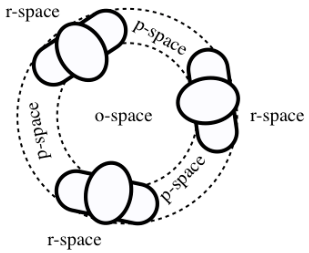
\includegraphics[width = 0.60\textwidth]{Figure/F-Formation} 
\caption{Illustration af en F-formation dannet af tre deltagere samt dens inddeling af områder, \parencite[s. 446]{PDF:UsingFFormations}.}
\label{fig:F-Formation}
\end{figure}
\noindent 
%
På \autoref{fig:F-Formation} illustreres en F-formation bestående af tre mennesker. Mennesker danner et område kaldt \textit{transactional segment}, hvor både opmærksomheden dirigeres hen og hvor objekter manipuleres. Størrelsen på dette område afhænger af aktiviteten men afhænger af underkroppens position, \parencite[s. 446]{PDF:UsingFFormations}. Når to eller flere menneskers \textit{transactional segment} overlapper hinanden dannes der et fælles \textit{transactional segment}, kaldt \textit{o-space}, hvor alle har lige tilgang, \parencite[s. 446]{PDF:UsingFFormations}. \textit{O-space} illustreres på \autoref{fig:F-Formation}. Området mellem menneskerne kaldes \textit{p-space} og området omkring F-formationen kaldes \textit{r-space}, jævnfør \autoref{fig:F-Formation}. \textit{R-space} er det område hvor en robot vil befinde sig før den inkluderes i de rejsendes interaktion og derfra selv indgår i F-formationen. Størrelsen af \textit{o-space} afhænger derfor af hvor mange der deltager i interaktionen, og hvordan dette område tilpasser sig efter spatial og holdningsmæssig adfærd blandt de deltagende, \parencite[s. 446]{PDF:UsingFFormations}. Udover den cirkulære F-formation afbilledet på \autoref{fig:F-Formation}, kan formationen ligeledes gengive en halvcirkel eller en rektangel, såfremt der er minimum tre interaktionspartnere involveret, \parencite[s. 446]{PDF:UsingFFormations}.   
%

\subsubsection*{Robottens hastighed}
\label{InteraktionSocialeRobotterParametreBevaegelsesmoenstreHastighed}
%
Ifølge \textcite[s. 165]{PDF:HumanRobotEmodiedInteraction} er den normale ganghastighed for et menneske mellem 3.6 km/t og 7.2 km/t, hvorfor det må forventes at en social robot ikke bør overskride det interval ved HRI. I undersøgelsen foretaget af \textcite[s. 175]{PDF:HowMayIServeYou} varierede robottens hastighed sig mellem 0.9 km/t og 1.44 km/t, hvor 60 \% af testpersonerne angav at hastigheden var \textit{about right} og 40 \% angav at hastigheden var for langsom. Ifølge \textcite[s. 178]{PDF:HowMayIServeYou} bør en robot, efter en tilvænningsperiode eller efter behov, bevæge sig hurtigere end 1.44 km/t. 

I undersøgelsen foretaget af \textcite[s. 169]{PDF:HumanRobotEmodiedInteraction} svinger robottens gennemsnitlige hastighed mellem 0.9 km/t og 1.4 km/t. Årsagen til at robottens gennemsnitlige hastighed ikke er højere skyldes, at når robotten passerer et menneske sænkes hastigheden, \parencite[s. 169]{PDF:HumanRobotEmodiedInteraction}. Baseret på testpersonernes vurdering af robottens hastighed ville en højere hastighed være at foretrække, \parencite[s. 169]{PDF:HumanRobotEmodiedInteraction}. Ydermere tyder det på, at robottens lave hastighed blev perciperet som værende mindre sikker og tilmed irriterende, \parencite[s. 169]{PDF:HumanRobotEmodiedInteraction}, hvorfor der bør anvendes en højere hastighed. For at afgøre hvilken hastighed robotten bør bevæge sig med argumenterer \textcite[s. 167]{PDF:HumanRobotEmodiedInteraction} for, at robotten bør være i stand til at tilpasse sin hastighed afhængigt af menneskets hastighed, da dette vil medføre en mere dynamisk interaktion mellem robot og menneske. Ifølge \textcite[s. 1897]{PDF:NavigationForHRITasks} bør robotten sænke hastigheden når den nærmer sig en gruppe af mennesker, ligesom et menneske ville gøre det, hvis det nærmede sig en gruppe af mennesker.

\textcite[ss. 192-103]{PDF:PsychologicalEffects} undersøger tre forskellige hastigheder, fordelt på to måder robotten kan nærme sig et menneske på. Robotten kan enten nærme sig direkte eller indirekte, ved direkte er hastigheden enten 0.91 km/t eller 3.66 km/t og ved indirekte er hastigheden 1.83 km/t, \parencite[ss. 192-103]{PDF:PsychologicalEffects}. En indirekte tilgang gengiver, at robotten først drejer mod venstre og derefter mod højre, hvilket giver en fornemmelse af at robotten bevæger sig en anelse til højre for mennesket, \parencite[s. 193]{PDF:PsychologicalEffects}. Med udgangspunkt i robottens hastighed fandt \textcite[s. 196]{PDF:PsychologicalEffects}, at den direkte hastighed på 3.66 km/t var ubehagelig og at den indirekte hastighed på 1.83 km/t var at foretrække, da den var mest behagelig. \blankline  
%
Baseret på de tre undersøgelser tyder det på, at hastigheder til og med 1.44 km/t i nogen grad kan accepteres, men det vil være, at foretrække hvis hastigheden var højere. Eftersom 1.44 km/t er langsommere end menneskets normale ganghastighed bør det være muligt, at øge robottens hastighed uden det påvirker interaktionen med mennesket negativt. Det lader rent faktisk til, at en øget hastighed potentielt kan forbedre interaktionen mellem robot og menneske, hvorfor der bør tages højde for dette. Dog tyder det på at robottens hastighed ikke må overstige mennesket normale ganghastighed.       
%

\subsubsection*{Robottens udseende og personlighed}
\label{InteraktionSocialeRobotterParametreBevaegelsesmoenstreUdseende}
%
Ifølge \textcite[s. 226]{PDF:SocailAndCollaborative} behøver en social robot ikke at have en menneskelignende krop, da bare det at robotten bevæger sig på en ikke-forudsigelig måde kan få mennesker til at percipere robotten, som havende en intention og en personlighed, jævnfør antropomorfisering. Dette hænger formentligt sammen med hypotesen omkring \textit{Uncanny Valley} fremsat af \textcite{PDF:UncannyVally}. Hypotesen bygger på hvilken effekt robottens udseende har på det tilhørsforhold mennesket oplever, hvor tilhørsforholdet kraftig forringes hvis robotten afspejler alt for menneskelige træk, både i forhold til udseende og bevægelse, \textcite{PDF:UncannyVally}. Ydermere argumenterer \textcite[s. 610]{PDF:SpencerProject} for, at hvis robottens udseende er alt for menneskeligt vil det øge brugerens forventninger til systemet vedrørende robottens kognitiveegenskaber. Dette kan lede til at brugeren bliver skuffet eller nægter at interagere med robotten, \parencite[s. 610]{PDF:SpencerProject}. I tillæg pointerer \textcite[s. 226]{PDF:SocailAndCollaborative}, at robottens størrelse, form, farve og bevægelsesmønstre har en indflydelse på hvordan robotten perciperes. \blankline
%
\textcite[s. 189]{PDF:PsychologicalEffects} præsenterer deres testpersoner for en cylinder-formet robot med og uden krop. Højden med krop er omkring 170 cm, hvor højden uden kroppen er 35 cm, \parencite[s. 189]{PDF:PsychologicalEffects}. De finder, at når robotten har en krop får det testpersonerne til at føle sig mere ukomfortable, både i forhold til hvordan robotten skal nærme sig, direkte eller indirekte, og hvor kort afstanden mellem robot og menneske må være, sammenlignet med robotten uden krop, \parencite[s. 196]{PDF:PsychologicalEffects}. Dog kan det ikke tydes ud fra resultaterne, hvorvidt det udelukkende er robottens højde eller robottens menneskeagtige krop, der får testpersonerne til at føle sig ukomfortable.   

En undersøgelse som forsøger at holde udseendet konstant og varierer højden, er udført af \textcite[s. 255]{PDF:RecommendationEffects}. Den lille robot er omkring 30 cm høj, hvor den store robot er omkring 120 cm høj. Ifølge \textcite[s. 255]{PDF:RecommendationEffects} har robottens størrelse indflydelse på \textit{attractiveness} og \textit{ease of initiating interaction}. Begge robotter implementeres i et Japansk storcenter og har til formål at printe rabatkuponer ud til de besøgende samt agere vejviser, \textcite[s. 252]{PDF:RecommendationEffects}. Baseret på resultaterne henvendte flere besøgende sig til den lille robot for at starte interaktionen, sammenlignet med den store robot, \parencite[s. 260]{PDF:RecommendationEffects}. I tillæg kommenterer \textcite[s. 260]{PDF:RecommendationEffects}, at den store robot kan virke skræmmende særligt for børn.\blankline
%
Ifølge \textcite[s. 226]{PDF:SocailAndCollaborative} har robottens personlighed indflydelse på hvor meget mennesker stoler på dens instruktioner. Robottens personlighed skal endvidere stemme overens med hvilke opgaver den skal løse, hvori situationer hvor robotten skal anvendes som underholdningsmiddel, er det en fordel at den udstråler glæde og humor, modsat situationer hvori opgaven er mere alvorlig, hvor robotten bør udstråle seriøsitet, \parencite[s. 226]{PDF:SocailAndCollaborative}. Selvom mennesker foretrækker en glad robot er de mere tilbøjelige til at følge instruktioner, hvis de leveres af en seriøs robots, \parencite[s. 226]{PDF:SocailAndCollaborative}. En måde hvorpå robottens personlighed kan komme til udtryk er via gestikker, som kan få robotten til at afspejle menneskelige følelser, såsom at være genert, tilbageholdende eller beskeden, \parencite[s. 227]{PDF:SocailAndCollaborative}. Ved hjælp af gestikker er det muligt for robotten at give interaktionspartneren feedback, eksempelvis i form af at nikke med hovedet for at indikere, at en kommando er forstået, \parencite[s. 228]{PDF:SocailAndCollaborative}.

Med udgangspunkt i \textcite[s. 272]{PDF:PersonalityOfSocialRobots} er de to vigtigste, ud af \textit{the big five}, personlighedskarakteristikas \textit{extroversion} og \textit{agreeableness}, eller venlighed og dominans, i forhold til sociale interaktioner. Dominans kommer blandt andet til udtryk ved en ret holdning, modsat en mere underdanig personlighed, som kommer blandt andet kommer til udtryk ved en mere krum holdning, \textcite[s. 273]{PDF:PersonalityOfSocialRobots}. Baseret på resultaterne fremgår det, at robotter med et mere menneskeligt udseende; bestående af to øvre kropslegemer, en overflade som afspejler en form for hud, en blanding af varme og kolde farver samt en form for beklædning, perciperes som værende mere venlig end robotter som kun har et øvre kropslegeme, en mere metallisk overflade, kolde farver og uden beklædning, \textcite[s. 275]{PDF:PersonalityOfSocialRobots}.

\section{Miniprojekt omhandlende vinkel på robot hovede}
Det følgende er et miniprojekt udført i forbindelse med et kurses kørt af Christian Sejr Pedersen kaldet Applied Experimental Psychology and Psychophysics. Formålet var at teste to skalaer mod hinanden. Vi valgte at tage udgangspunkt i Karls robot vha. den lo-fi prototype, der er bygget.

\subsection*{Skaleringseksperiment}
Målet med dette eksperiment er at undersøge om robottens hovedposition har indflydelse på hvor indbydende testpersonerne perciperer robotten. Hovedpositionen kan være med til at signalere hvilket stadie robotten er i så brugeren ikke er i tvivl om, hvorvidt robotten henvender sig til dem for en mulig interaktion eller om robotten er utilgængelig. Hvor indbydende robotten perciperes angives på en skala.

\subsection*{Testdesign}
%
Til testen anvendes en visuel prototype af robotten, som er illustreret på \autoref{fig:position}. Testpersonerne bliver præsenteret for de fire forskellige hovedepositioner; position 1, som er 100$^{\circ}$, position 2, som er 65$^{\circ}$, position 3, som er 35$^{\circ}$, samt position 4, som er 0$^{\circ}$. De fire forskellige positioner er præsenteret på \autoref{fig:position}.   
%
\begin{figure}[H]
\centering
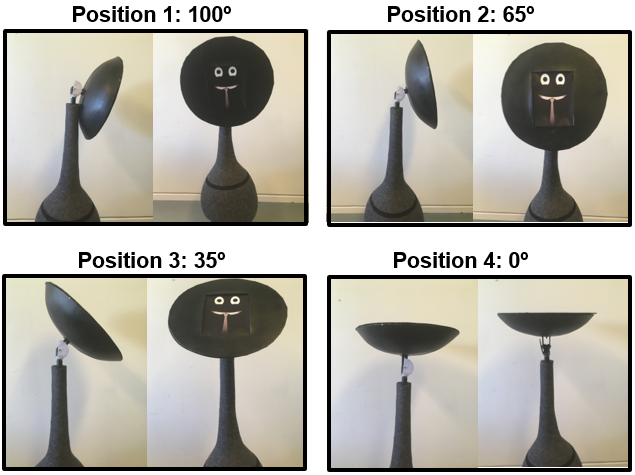
\includegraphics[width = \textwidth]{Figure/positionerBilleder.PNG} 
\caption{De fire valgte hovdepositioner.}
\label{fig:position}
\end{figure}
\noindent 
%
For at balancere stimulipræsentationen anvendes et \textit{Latin Square Design}, hvilket giver fire mulige kombinationer hvorved stimuli præsenteres i. Stimuli defineres som værende robottens hovedposition. For at indsamle mere data bliver hver kombinationsmulighed præsenteret to gange, hvilket medfører at der i alt vil blive indsamlet data fra otte testpersoner. Præsentationsrækkefølgen fremgår af \autoref{tab:Latin}.  
%
\begin{table}[H]
	\centering
	\begin{tabular}{l|c}
		Testperson     & Præsentationsrækkefølge for position \\\hline
		Testperson 1   & 1 - 2 - 3 - 4          \\\hline
		Testperson 2   & 2 - 3 - 4 - 1          \\\hline
		Testperson 3   & 3 - 4 - 1 - 2          \\\hline
		Testperson 4   & 4 - 1 - 2 - 3          \\\hline
		Testperson 5   & 1 - 2 - 3 - 4          \\\hline
		Testperson 6   & 2 - 3 - 4 - 1          \\\hline
		Testperson 7   & 3 - 4 - 1 - 2          \\\hline
		Testperson 8   & 4 - 1 - 2 - 3   
	\end{tabular}
	\caption{Præsentationsrækkefølgen for robottens fire hovedpositioner.}
	\label{tab:Latin}         
\end{table}
\noindent
%
Testen afvikles i forhallen på Frederik Bajers vej 7H, for at simulere et befolket område som eksempelvis en lufthavn. Dog udføres den ene af de to pilot tests i kantinen på Frederik Bajers vej 7.
%
\subsubsection*{Instruktioner}
\label{Instruktioner}
%
Testpersonerne får følgende instruktioner: 
%
\begin{quotation}
\noindent
Hej!\blankline
%
Fedt at du gider at hjælpe os. Du skal forestille dig, at det her er en robot. Lige nu kan den ingenting. Det er meningen at robotten skal indgå i en lufthavn, hvor der er mange mennesker. Hovedet vil blive indstillet i fire forskellige positioner og du skal derfra angive, hvor indbydende du synes robotten er. Det gør du på en skala fra slet ikke til ekstremt indbydende.\blankline
%
Har du nogen spørgsmål?
\end{quotation}
%
Derefter præsenteres testpersonen for de fire forskellige hovedpositioner i den specifikke rækkefølge, jævnfør \autoref{tab:Latin}. Efter hver præsentation udleveres en skala hvorpå testpersonen, med en kuglepen, angiver hvor indbydende de synes robotten var i netop den position.  
%

\subsubsection*{Design af skala}
%
Testpersonerne bliver til hver af de fire hovedpositioner spurgt om: \textit{Hvor indbydende synes du robotten er?}, hvortil testpersonerne angiver sin respons på en \textit{Visual Analog Scale} (VAS). Skalaen er opstillet med åbne endepunkter samt to ankerpunkter placeret 1,5 cm fra hvert endepunkt, skalaen er illustreret på \autoref{fig:VAS}. Venstre ankerpunkt er angivet med \textit{Slet ikke}, modsat det højre ankerpunkt, som er angivet med \textit{Ekstremt}. Ved at vælge en VAS med åbne endepunkter har testpersonerne mulighed for, at overgå sig selv i tilfælde af, at de perciperer robotten som værende endnu mere indbydende end den mest indbydende robot de hidtil har været udsat for. Ved at designe skalaen med åbne endepunkter undgåes ophobning af respons omkring endepunkterne. 
%
\begin{figure}[H]
\centering
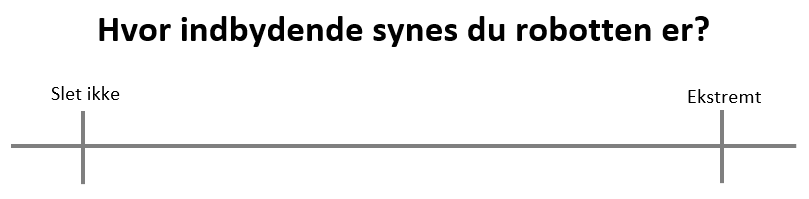
\includegraphics[width = 0.8\textwidth]{Figure/VAS.PNG} 
\caption{Illustration af den designede VAS med åbne endepunkter og med de angivne ankerpunkter, samt spørgsmålet som testpersonerne skal svare på.}
\label{fig:VAS}
\end{figure}
\noindent 
%
\subsection*{Hypotese}
\label{Hypotese}
%
Formålet med eksperimentet er, at undersøge om der er forskel på hvor indbydende robotten perciperes afhængigt af hvordan robottens hovede er positioneret. Baseret på de fire valgte positioner, jævnfør \autoref{fig:position}, kan følgende hypotese formuleres: 
%
\begin{quotation}
\noindent
  \textit{Når robottens hovede befinder sig i position 2 eller position 3 perciperes robotten mere indbydende end når hovedet befinder sig i position 1 eller position 4.}
\end{quotation}
\noindent
%
Med udgangspunkt i ovenstående hypotese kan den alternative hypotese, $H_a$, opstilles:
%
\begin{quotation}
\noindent
\begin{equation}
  H_a: Position 2 \wedge Position 3 > Position 1 \wedge Position 4
\end{equation}  
\end{quotation}
\noindent
%
Med udgangspunkt i den alternative hypotese, $H_a$, kan følgende nul hypotese, $H_0$, opstilles: 
%
%
\begin{quotation}
\noindent
\begin{equation}
  H_0: Position 2 = Position 3 = Position 1 = Position 4
\end{equation}  
\end{quotation}
\noindent
%
\vfill

\subsection*{Pilottest}
\label{Pilottest}
%
I forbindelse med at udvikle skalaer er det vigtigt, at sikre sig at skalaerne fungerer og at testpersonerne er i stand til anvende dem. Formålet med pilottesten er derfor ikke at undersøge hvor indbydende robotten perciperes, men derimod at undersøge om testpersonerne er i stand til at anvende den designede VAS og dertil om de forstår de angivne ankerpunkter. \blankline
%
Foruden instruktionerne, der fremgår i \fullref{Instruktioner}, bliver testpersonerne i pilottesten ydermere spurgt om:\blankline   
%
\begin{itemize}
	\item Kan du forstå hvordan du skal bruge skalaen?
	\item Hvordan synes du det var at bruge skalaen?
	\item Havde du nogen problemer med at forstå skalaen?
	\item Kunne du forstå de to labels på skalaen?
	\item Kunne du forstå spørgsmålet?
	\item Har du andre kommentarer?
\end{itemize} 
%
Pilottesten blev afviklet med to testpersoner; to mandlige studerende på Aalborg Universitet. Den første pilottest blev afviklet i kantinen på Frederik Bajers vej 7, hvorefter de restende tests blev afviklet i forhallen på Frederik Bajers vej 7H. 
%
\subsubsection*{Databehandling af pilottest}
%
Baseret på testpersonernes respons var det klart hvordan skalaen skulle anvendes og der opstod hverken problemer med at bruge eller forstå skalaen, når testpersonerne skulle angive hvor indbydende robotten var. I tillæg gav testpersonerne udtryk for at spørgsmålet: \textit{Hvor indbydende synes du robotten er?} var letforståeligt. I henhold til spørgsmålet omkring hvorvidt testpersonerne kunne forstå de angivne labels, gav testpersonerne udtryk for at det ikke var et problem at forstå dem. 

Dog gav testperson 1 udtrykt for nok aldrig at ville bruge udtrykket \textit{ekstremt indbydende} om en robot, da udtrykket forbindes med at være attraktiv, hvilket testpersonen ikke synes en robot er. På trods af denne kommentar vælges det at bibeholde \textit{Ekstremt}, som det højre ankerpunkt.

I forhold til skalatype, gav testperson 2 udtryk for bedre at kunne lide en kontinuerlig skala, hvilket VAS er, fremfor en skala, der er punktopdelt. Hvilket kommer til udtryk ved følgende kommentar:
% 
\begin{quotation}
  \textit{[...] synes den her skala er bedre end sån en 1-10 skala.}, testperson 2.
\end{quotation}


\subsection*{Resultater}
\label{Resultater}
%
Testen blev udført på otte testpersoner; tre kvinder og fem mænd, med et aldersspænd fra 21 år til 34 år (gennemsnit: 24,6 år). Testpersonerne er alle studerende på Aalborg Universitet fordelt på følgende studieretninger: Jura, Kemi-Teknologi, Fysisk og Biologi.\blankline
%
På \autoref{fig:RaaDataTestpersoner} fremgår de otte testpersoners individuelle vurderinger af, hvor indbydende robotten perciperes afhængigt af hovedposition.  
%
\begin{figure}[H]
\centering
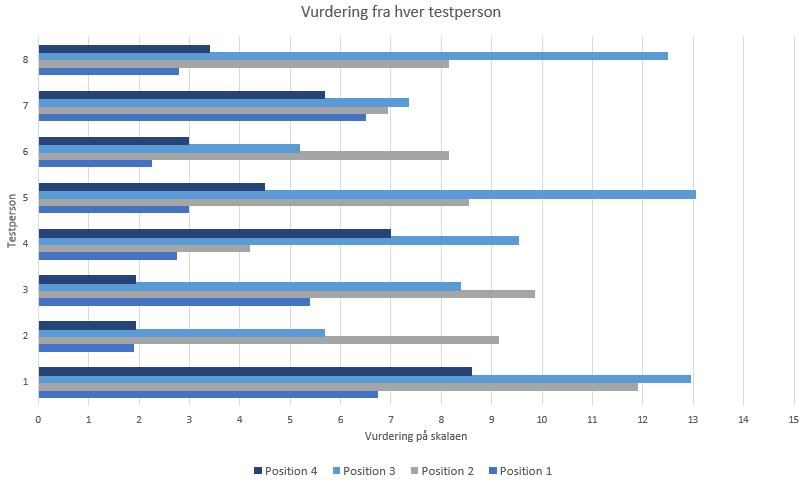
\includegraphics[width = \textwidth]{Figure/RaaDataTestpersoner.PNG} 
\caption{Rådata fra hver testperson. X-aksen er defineret ud fra den definerede skala-længde, hvorfor x-værdierne afspejler hvor indbydende testpersonen perciperer robotten. Testpersonerne er angivet på y-aksen.}
\label{fig:RaaDataTestpersoner}
\end{figure}
\noindent
%
\autoref{fig:RaaDataPositioner} er en sorting af data, som afspejler hvor indbydende hver testperson perciperer den specifikke hovedposition. 
%
\begin{figure}[H]
\centering
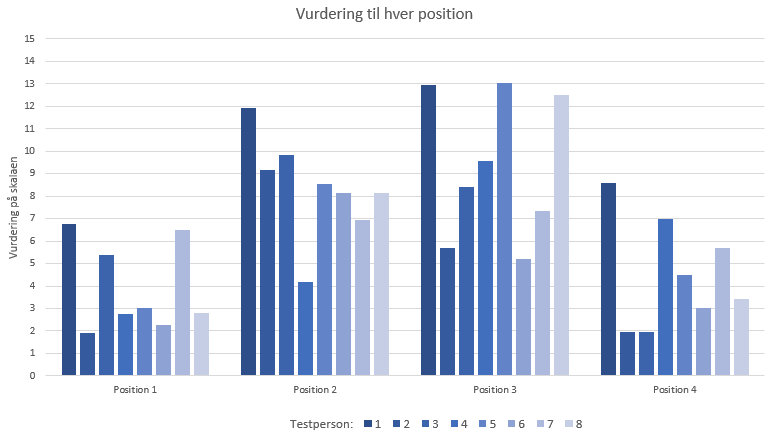
\includegraphics[width = \textwidth]{Figure/RaaDataPositioner.PNG} 
\caption{Rådata sorteret efter de fire hovedpositioner, repræsenteret på x-aksen, hvor y-aksen gengiver hvor indbydende hver testperson perciperer robotten afhængigt af hovedposition.}
\label{fig:RaaDataPositioner}
\end{figure}
%
Med udgangspunkt i \autoref{fig:RaaDataPositioner} tyder det på, at både position 2 og position 3 perciperes som værende mere indbydende end både position 1 og position 4.\blankline
%
For at besvare hypoteserne, opstillet i \fullref{Hypotese}, vil der i følgende afsnit udføres statistiske analyser.   


 \subsection*{Analyse}
\label{Analyse}
%
Før analysen udføres, opstilles et boksplot for hver af de fire hovedpositioner, jævnfør \autoref{fig:boksplot}. Baseret på \autoref{fig:boksplot} tyder det på, at position 2 og position 3 begge perciperes som værende mere indbydende sammenlignet med position 1 og position 4.   
%
\begin{figure}[H]
\centering
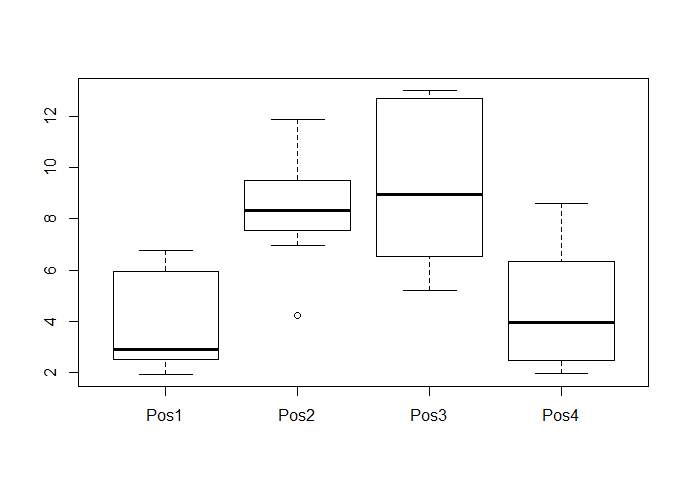
\includegraphics[width = 0.7\textwidth]{Figure/Rplot.png} 
\caption{Boksplot over hvor indbydende hver af de fire hovedpositioner perciperes.}
\label{fig:boksplot}
\end{figure}
\noindent
%
Data analyseres med en \textit{One-way Repeated Measures ANOVA}. Hvor \textit{one-way} refererer til antallet af uafhængige variable, som i dette tilfælde er én; robottens hovedposition. \textit{Repeated measures} refererer til, at samtlige testpersoner præsenteres for samtlige stimuli. Da formålet med denne test er at undersøge hvor indbydende en robot perciperes afhængigt af dens hovedposition, er den afhængige variabel testpersonernes individuelle respons angivet på skalaen. Den indsamlede data er af typen interval data, hvilket skyldes at VAS er en kontinuerlig skala. 

Ydermere dækker den uafhængige variabel over fire kategorier; de fire forskellige hovedpositioner, er det ligeledes oplagt at anvende en ANOVA, da det ønskes at sammenligne mere end to kategorier.\blankline
%
Følgende antagelser skal overholdes for at udføre en \textit{One-way Repeated Measures ANOVA}, \parencite[ss. 575-577]{DiscoveringStatisticsUsingR}: \blankline  
%
\begin{itemize}
	\item \textbf{Den afhængige variabel skal som minimum være målt på interval skala.}\\
	Vurderingen givet på skalaen er målt på en interval skala og opfylder dermed denne antagelse.
	\item \textbf{Der skal være homogen varians. }\\
	For at teste om der er homogen varians udføres \textit{Levene's test}. Testresultatet er $F(3.28)=1.09, p=0.37$, hvorfor der ikke er signifikant forskel og dermed er antagelsen om homogen varians opfyldt. 
	\item \textbf{Data skal være normalfordelt.}\\
	For teste om der er normalfordeling udføres en \textit{Shapiro-Wilk test}. Testresultatet er $W=0.94, p=0.09$, hvorfor der ikke er signifikant forskel og dermed er antagelsen om normalfordeling er opfyldt.
	\item \textbf{Uafhængig data.}\\
	Testpersonernes respons er uafhængige; testperson 1 har ikke indflydelse på de resterende testpersoners respons. Dog er der afhængighed mellem de fire konditioner testpersonerne præsenteres for.\blankline
\end{itemize}
\noindent
%
Da alle antagelser for at udføre en \textit{One-way Repeated Measures ANOVA} er opfyldt, udføres denne i \textit{rStudio}. Testresultatet er $F(3.21)=13,7, p=4.4*e^{-4}$, hvilket indikerer at der er signifikant effekt af robottens hovedposition på hvor indbydende robotten perciperes.

Baseret på dette resultat er det kun muligt at konkludere, at der er signifikant forskel mellem hvordan hovedpositionerne perciperes i forhold til hvor indbydende robotten er, det er derfor ikke muligt at afgøre hvor den signifikante forskel er. For at undersøge hvor forskellen er udføres der en \textit{Post Hoc test} af typen \textit{Pairwise Comparison}, hvilket udføres med t-tests, \parencite[s. 1338]{DiscoveringStatisticsUsingR}. Testresultatet fremgår af \autoref{fig:sammenligning}.
%
\begin{figure}[H]
\centering
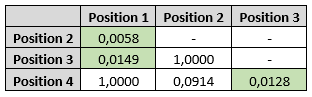
\includegraphics[width = 0.5\textwidth]{Figure/PostHocExcel.PNG} 
\caption{Sammenligning mellem vurderingerne af hvor indbydende robotten perciperes i henhold til dens hovedposition. Grøn markering angiver signifikante forskelle.}
\label{fig:sammenligning}
\end{figure}
\noindent
%
Baseret på \autoref{fig:sammenligning} fremgår det at både position 2 og position 3 er signifikant forskellige fra position 1. Sammenholdes dette med \autoref{fig:boksplot} kan det konkluderes at både position 2 og position 3 perciperes som værende mere indbydende end position 1. I tillæg er der signifikant forskel mellem position 3 og position 4, hvor position 3 perciperes som værende mere indbydende. Det er dog bemærkelsesværdigt at det ikke er tilfældet mellem position 2 og position 4, hvor der ikke fremgår en signifikant forskel, jævnfør \autoref{fig:sammenligning}.
%

\subsection*{Diskussion}
\label{Diskussion}
%
Foruden information omkring køn, alder og studieretning kunne det have været en fordel at måle testpersonernes højde, da den ene af testpersonerne, baseret på testledernes vurdering, var betydeligt højere end de resterende, samt en testperson, som var betydeligt lavere end de restende testpersoner. Disse højdeforskellen kan potentielt have en indflydelse på hvor indbydende testpersonerne perciperede robotten afhængigt af dens fire hovedpositioner. 

Under en samtale antages det, at samtalepartnerne generelt vil søge efter at opnå øjenkontakt og opretholde en form for øjenhøjde. Er dette tilfældet kan det ligeledes antages at robottens hovedposition positionelt har indflydelse på, hvorvidt testpersonerne betragter robotten som en form for samtalepartner og ydermere hvilke interaktionsmuligheder robotten tillader. Det vil derfor være interessant at undersøge sammenhængen mellem brugerens højde og hvor indbydende robotten perciperes afhængigt af hovedposition.\blankline  
%
Testpersonerne angav på en \textit{Visual Analogue Scale} (VAS), hvor indbydende de perciperede robotten afhængigt af dens hovedposition. Skalaen var designet med åbne endepunkter samt to ankerpunkter angivet med \textit{Slet ikke} og \textit{Ekstremt}. Som tidligere nævnt kommenterede testperson 1 i pilottesten at ankerpunktet \textit{Ekstremt} ikke var det mest passende ord at anvende som label, da det for testpersonen forbindes med at være attraktiv, hvilket testpersonen gav udtryk for robotter ikke er. Selvom det blev vurderet ikke at ændre på skalaen, kunne det have været en fordel at udføre gentagende pilottests for at undersøge om andre har en lignende holdning og på baggrund af det ændre labelen.    

Ydermere kan ordet \textit{ekstremt} også betragtes som værende et negativt ladet ord i den forstand, at det oftest benyttes til at beskrive kraftige vejrforhold, naturkatastofer eller politiske holdninger langt fra, hvad der antages for normalt, \parencite{WEB:Oxford2017}. Det kunne derfor have været en fordel at undersøge om der kunne findes en erstatning for \textit{Ekstremt} på den anvendte skala. Dog er en af fordelene ved at vælge et ord som \textit{Ekstremt}, at der formentlig ikke vil forekomme stimuli, der er endnu mere ekstreme end før. Taget i betragtning af at det andet ankerpunkt er \textit{Slet ikke}, hvor der det er svært at finde et alternativ som er mindre end slet ikke, så er det oplagt at vælge et ord til det andet ankerpunkt som dækker det samme. Med de to valgte ankerpunkter har det været muligt at dække hele skalaen, hvor hvis der var brugt \textit{Slet ikke} og \textit{Meget}, så ville der potentielt være stimuli som er mere end meget, hvorfor der formentlig vil forekomme samlinger omkring endepunktet, hvilket ikke har været tilfældet med de to valgte ankerpunkter.\blankline
%
Testpersonerne blev bedt om at vurdere hvor indbydende de perciperede robotten til hver af de fire hovedpositioner, hvor der antages en fælles forståelse for ordet \textit{indbydende}. Det blev observeret af testlederne, at et par af testpersonerne spurgte ind til hvad der mentes med indbydende, hvor testlederne var nødsaget til at uddybe forklaringen. En måde hvorpå der kunne skabes en form for fællesforståelse kunne have været, at præcisere yderligere hvor robotten er tiltænkt samt hvad dens formål er. Det kunne have indebåret en opgave, som testpersonerne skulle løse ved hjælp af robottens ansigt, som i det tilfælde skulle erstattes med en touchskærm. Ved at anvende en touchskærm kunne det potentielt have medvirket dels til en fælles forståelse for ordet \textit{indbydende} men også en forståelse for hvordan interaktionen med robotten foregår. \blankline
%
Testen blev kun udført af otte testpersoner, hvilket har indflydelse på præcisionen af de statiske analyser. Dette afspejles blandt andet af den store variation i respons, særligt ved position 2 og position 4, jævnfør \autoref{fig:boksplot}. Havde flere testpersoner deltaget kunne det have medført en mere pålidelig sammenhæng mellem hvor indbydende robotten perciperes afhængigt af dens hovedposition. 



\subsection*{Konklusion}
\label{Konklusion}
%
Position 2 (65$^{\circ}$) og position 3 (35$^{\circ}$) blev begge vurderet til at være mere indbydende end position 1 og position 4, som generelt blev vurderet på skalaens nedrehalvdel. Der blev udført en \textit{One-way Repeated Measures ANOVA}, som indikerede at der forekommer en signifikant forskel mellem hovedpositionerne i forhold til hvor indbydende robotten perciperes. Efterfølgende blev der foretaget en \textit{Pairwise Comparison}, hvorfra det blev fundet, at der er signifikant forskel mellem position 1 og position 2, mellem position 1 og position 3, samt en forskel mellem position 3 og position 4. Baseret på resultaterne er det muligt at afvise nul hypotesen, $H_0$, jævnfør \fullref{Hypotese}. Der er dog ikke endegyldigt belæg for at acceptere den alternative hypotese, $H_a$, da der ikke er fundet en signifikant forskel mellem position 2 og position 4. 

Dog kan det konkluderes, at for at robotten perciperes mest indbydende, i forhold til de fire valgte hovedpositioner, skal den være indstillet enten i position 2 eller i position 3. Dette gengiver at robottens hovede er vinklet skråt opad, hvilket formentlig giver testpersonerne i følelse af, at de har øjenkontakt med den.       

